\chapter{Design}

Having looked at other related solutions in the problem area and mentioning their
interesting points and weaknesses, we now turn our attention to the design of our own solution.
It was decided that we would design an alternate system based upon the Kademlia
Distributed Hash Tablet (DHT). We will take inspiration from parts of several of the systems
mentioned in the Related Work subsection.

Our design will consist of several users in a distributed system, which we refer to as “nodes”,
each with the same capabilities. Each node will contribute to the network by serving some of the
content that other users publish.

We will now discuss the reasoning and arguments behind design choices made in the architecture of this system,
and then provide a description of system design.

\section{Design Choices}

\subsection{Author Anonymity}

In order for an author of some web content to remain anonymous, they must not have any connection
to that content. This introduces a number of complications for web serving. If a user does not want
to be associated with content that they wish to publish, they can not hold that content. This means
that content must be held by other users in the system.

\subsubsection{Peer-to-Peer}
A peer-to-peer computer network is a network in which all nodes contribute some resources to the
network as a whole. These resources can be, for example, disk space, computing power, or bandwidth.
The nodes on a peer-to-peer network all have the same functional capabilities in the network.

A peer-to-peer network was chosen for the underlying network of this system. Users of the system will
contribute disk space and internet bandwidth to assist in the running of the network. This disk space and
internet bandwidth will be used to provide other users access to web-page data on the network. Users in
the network are identified by a numeric “node ID”.

\subsubsection{Anonymity}
Author anonymity can be achieved by distributing an author's content to other users in the network.
This way, users that wish to read content written by a certain user do not make any connections to that user.

%%%%%%%%%%%%%%%%%%%%%%%%%%%%%%%%

\subsection{Reader Privacy}

\subsubsection{Traffic Analysis}

Traffic tracking by ISPs can be done through analysing the destination address in an IP packet. To avoid this,
the system should avoid direct connections between a user and a website. This is achieved through a multi-hop
peer-to-peer network. This is used avoid direct connections between a user that hosts content and the user
requesting that content. With no direct connections between the content provider and reader, malicious third
parties can not make accurate assumptions about what a user is viewing based on the servers that they connect to.

\begin{figure}[H]
    \centering
    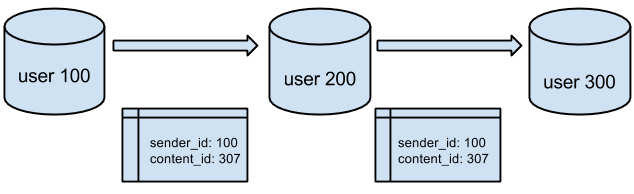
\includegraphics[width=0.8\textwidth]{img/indirection.png}
    \caption{Diagram demonstrating the use of a multi-hop peer-to-peer network to avoid user traffic tracking.
    Since user 100 contacts user 300 via user 200, no direct correlation between user 100 and user 300 can be made
by a third party analysing user 100's traffic.}
    \label{fig:multi-hop}
\end{figure}

There is a possibility of a compromise of reader privacy when a user receives the contents of a web-page which
they wish to view. If a malicious third party such as their Internet Service Provider or a rogue user on their
network were to intercept a user's traffic, they could view the web-content that a user has requested and use this
information to violate their privacy. To prevent this attack, we can encrypt web content in transmission. Thus, any
attacker that can intercept user traffic could only see encrypted data, and not the actual content that a user has
requested.

\subsubsection{Cryptography}

Each web-page in the system consists of three components apart from its content: a randomly generated unique
identifier (called a UUID), a “content location”, and cryptographic keys which we use to encrypt and decrypt web-page data.
We will now briefly discuss these terms and their meanings.

\textbf{UUID}

A website's UUID is known only to the users that wish to retrieve this web-page. These UUIDs act as URLs, but instead of
being in a form similar to a traditional website (for example, www.example.com/hello), they appear as a random string of
alphanumeric characters. These identifiers serve only to identify the website and play the same role as a URL in the web as
it exists today. These UUIDs could be shared outside of the system, or they could be linked from another web-page in the system
such as a search engine or web-page indexing site, similar to the case with traditional URLs.

A web-page's UUID is used to derive both its content location, and cryptographic key. These transformations are one-way,
and it is not possible to derive a web-page's UUID from either its content location nor cryptographic key.

\textbf{Content Location}

A web-page's “content location” is a numeric value which determines the ideal node ID in the network at which this content
should be stored. The content location is derived from a web-page's UUID through a hashing function which transforms this unique
identifier into numeric index at which the content should be stored.

It is not guaranteed that a user with any given Node ID will be present on a network. As a result of this, the content should be
stored at the numerically closest node or nodes to the content location identifier.

\textbf{Cryptographic Key}

In order to avoid compromise of user privacy through traffic analysis by malicious third parties, web content being sent to users
on the network should be encrypted. The encryption of this data requires a cryptographic key.

It would be inconvenient for users of the system to hold a database of cryptographic keys relating to web-sites. It would also be
inconvenient for users to have to manually send cryptographic keys when sharing UUID links to other users. To avoid this, we derive
the cryptographic key from the web-page's own UUID.

A Key Derivation Function is a cryptographic function that takes an arbitrary string and can
deterministically generate a cryptographic key from it. ~\cite{kdf} Using a Key Derivation Function, we
can generate a cryptographic key to encrypt and decrypt web-page content from a web-site's UUID.
When sending a request for a web-page, a user must only reveal a hash of its UUID (in order to
find its content location). This means that the only detail of a user's request that is revealed to the network
is the content location of that website. Since it is not possible to derive either the web-page UUID nor the web-page
encryption key from this content location, it is impossible for a third party to conclude the web-content that a user
has requested.

\begin{figure}[H]
    \centering
    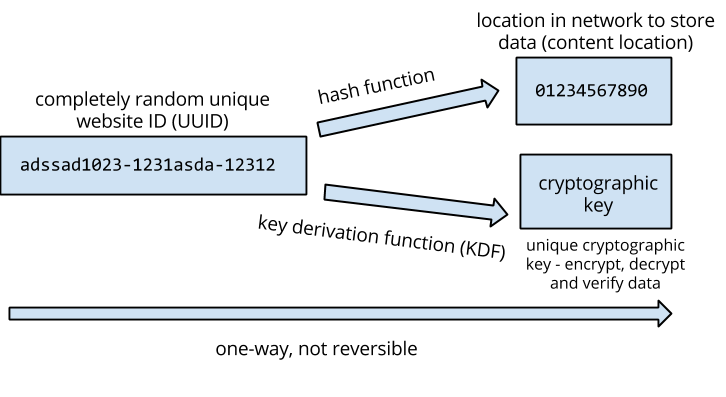
\includegraphics[width=0.8\textwidth]{img/KDF-hashing-example.png}
    \caption{Diagram of the derivation of the content-location and cryptographic key from a web-page UUID.}
    \label{fig:kdf_hashing}
\end{figure}


\subsubsection{Random sender ID replacement}


It is possible for a malicious user to join the network with the intention of analysing the
sender and destination ID fields in packets that they route through the network. All content request
packets routed through the network include both a sender ID and content ID field.

In Levacher's paper on “Elite” ~\cite{levacher}, he introduces a novel way of addressing this issue which we will use in this system.
All users, when passing a request on towards the destination, can randomly change the sender ID field in that message
to their own user ID and make a note that they have done so. When this user receives a response to this request,
they simply pass the message on to the original sender. This means that users in the network can not reliably tell
the real origin of a request, meaning that none of the users in the system can accurately record the activity of other users.

\begin{figure}[H]
    \centering
    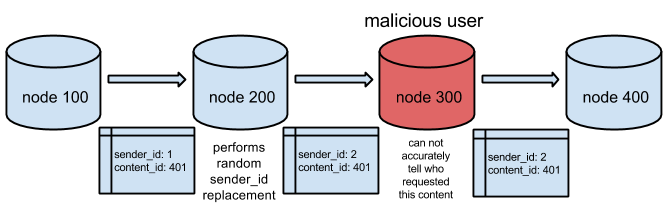
\includegraphics[width=0.8\textwidth]{img/sender_id.png}
    \caption{Diagram demonstrating the usage of random sender ID replacement used to hide the origin of a data request.}
    \label{fig:sender_id}
\end{figure}

%%%%%%%%%%%%%%%%%%%%%%%%%%%%%%%%%%%%%%%%%%%%%%%%%%%%%%%%%%%%%%%%

\subsection{Data Storage}


In order to preserve document anonymity, a user holding some data must not know what the data they is storing represents.
In the case of this system, this means that a user must not know what UUID a piece of data represents. It is also necessary for a
user to have no knowledge of the content that they store, so that they can not be held responsible for the actions of other users
of the system. Therefore, users should not be able to tell what the data they store represents, and should not be able to read the
data that they store.

Since content can not be held by its author in order to provide author anonymity, it is important that the legitimacy of stored data
can be verified by the users of the system. It must be possible for users to verify that the data which they receive has neither been
tampered with by the user holding it nor the users in the system that delivered the content to them. We will refer to this guarantee as
``content integrity''.

In this subsection, we will address and discuss these issues as well as provide techniques to provide provide them.

\subsubsection{Document Anonymity}

When a user is requested to hold a piece of data, they are told the content ID, which is an index in the network at which that data should
be stored, and the data to store.

The content ID of a piece of data is derived from the UUID of that data. To ensure that the content ID of a piece of data can not be determined,
the hash function of a UUID, u, to derive some content ID, c, must be irreversible. Therefore, the hash function used to derive a content ID
from a UUID must be sufficiently complex that it would be computationally infeasible to derive a UUID if given a content ID. ~\cite{sha1}

The data to be stored is encrypted by a cryptographic key derived from the UID of that data. The only way to determine what information to be
stored would be to use the cryptographic key to decrypt the data. This cryptographic key is derived, using a Key Derivation Function, from the UUID.

Since it should be computationally infeasible to derive the UUID of a piece of data from the content ID, it is impossible for a user to determine
either the contents of a piece of stored data or the web-page UUID which it represents.

\subsubsection{Content Integrity}

In order to guarantee content integrity, the system must provide a means of verifying that content stored in the system has not been modified
in any way. We can achieve this goal by using a cryptographic Message Authentication Code (MAC).

A Message Authentication Code is a cryptographic technique used for message authentication - that is, it is used to verify the authenticity of
a message. ~\cite{hmac} Given a message M and cryptographic key K, performing a MAC operation on K and M will generate an authentication code C. If a user
modifies M, it is computationally infeasible for a user that does not hold the secret key K to compute a MAC for this modified message. Thus,
if a user receives a response to a data request and the MAC does not verify the integrity of the contents of the received message, then the content
has been tampered with since its creation by the content's author and is not reliable.

\begin{figure}[H]
    \centering
    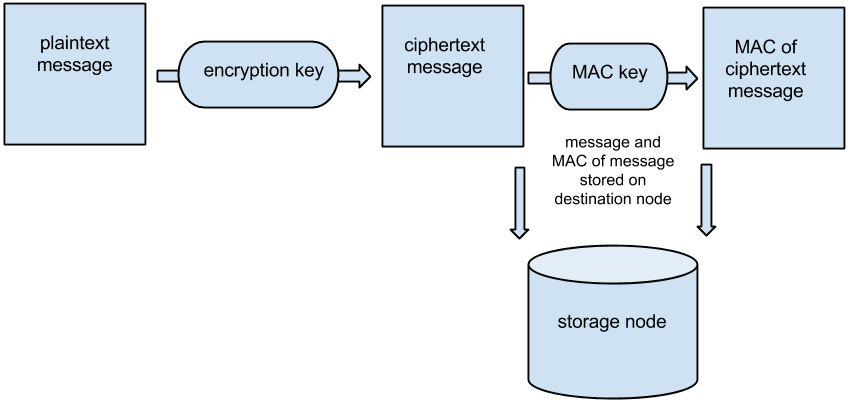
\includegraphics[width=0.8\textwidth]{img/mac.png}
    \caption{A diagram showing the process through which an secure cipher-text (encrypted) message and Message Authentication Code for that
    message is derived from a plain-text (unencrypted) message.}
    \label{fig:hmac}
\end{figure}


\subsection{Replication}


In order for the system to provide increased reliability and redundancy, data should be replicated across the network.
This will provide resilience against single node failure due to network problems, disk failure. By adding replication, we aim to
avoid a single-point-of-failure, providing increased reliability.

Kademlia networks provide automatic content replication ~\cite{kademlia}. In a Kademlia network, there is a global replication constant among all nodes
which determines the replication factor of the network. When some node N leaves the network, the other nodes that hold the replicas of
N's data automatically share the data that N held to the closest available nodes on the network.

We use Kademlia's built-in replication system to provide full document replication in the network.


\subsection{Censorship}

To provide community-driven censorship, the system must allow the users to make decide on the censorship of content on the system.

We will now discuss the difficulties associated with community consensus in a decentralised network and explain the
design choices made in this system to provide community-driven censorship.

\subsubsection{Decentralisation}

Since in this system there is no centralised service providing access to web-pages, censorship can not be controlled in one place.
Censorship on a web-page can also not be decided by the author of some content as this would enable users to never have their
content censored by the community.
Because of this, we propose that the censorship of web-pages should be done by the users that hold that web-page data.

\subsubsection{User-based content evaluation}

In ``Elite'', Levacher claims that users tend to browse web content that they are generally interested in. He also argues that if
a page is frequently viewed, then it must be of high-quality.

Levacher also makes an argument for a ``Zero-Input Recommendation System.'' Levacher's argument is that evaluating the quality of
content is most effective if users must exert no effort to do so. We argue then that if a users visits a web-page that they do not
object to, then the web-page must be of high quality. This implies that they agree with the content of the web-page and do not deem
it unsuitable for the community. Furthermore, if a user does visit a web-page that they object to, then they are likely to want it to
be removed from the system. These users must be given a means to voice their objection to this web-page.

In light of this, we propose a mixture of Levacher's ``Zero-Input Recommendation System'' combined with a channel for users to
report web-pages as unsuitable. We will allow users to send a notice of objection to a web-page, which we refer to as a `down-vote' in the
style of StackOverflow ~\cite{stackoverflow}. If a user views a web-page and does not send a `down-vote' about this page, then the
system assumes that a user does not object to the content and that the content is of high quality.

\subsubsection{``Downvote''-based Censorship}

In our system, we propose that censorship be decided by the aggregate ``up-vote'' minus ``down-vote'' value, where ``up-votes'' are implicitly
made when a user does not object to some content. We will now propose a novel algorithm for the removal of content.

Data in FreeNet is automatically pruned from the system once is not accessed in some time ~\cite{freenet}. This serves to remove old and unused
content from the network. We will borrow this idea in our system for the same reason. Web-pages will be given a time-to-live value (TTL),
which determines how long until they will be deleted from the system. Web-page accesses (implicit ``up-votes'') will increase this
TTL, whereas ``down-votes'' will decrease this value, meaning that content will be removed from the network sooner.

\subsubsection{Replication and Parallelisation Concerns}

Since Kademlia sends requests in parallel to all replicas that hold a piece of data in parallel, it is possible that a storage
node will receive a down-vote request from one user more than once. This is particularly important when the random sender ID
replacement occurs, as these down-vote requests are no longer individually discernible from each other. To counter-act this,
the down-vote request includes a unique identifier field (called ``downvote-UUID''). Once nodes receive a downvote request
with the same downvote-UUID as a previous request, the can assume that it is a repeat of a previous request and safely ignore it.

\section{System Design Overview}

\begin{figure}[H]
    \centering
    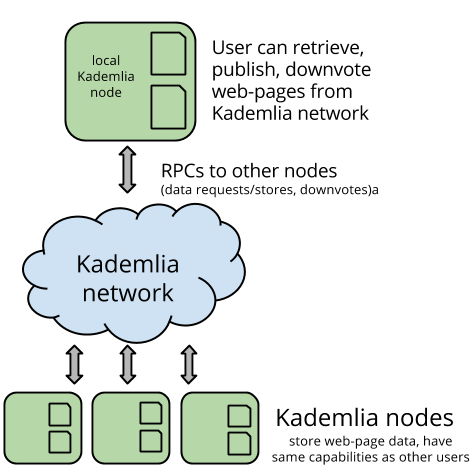
\includegraphics[width=0.6\textwidth]{img/arch.png}
    \caption{A diagram showing the system architecture.}
    \label{fig:arch}
\end{figure}

The system consists of several users (``nodes'') on a Kademlia network. There are three main actions that a user can perform,
with the necessary parameters in brackets:

\subsection{Web-page retrieval and verification}

To retrieve a web-page for a given UUID, the user must derive the content location from the UUID using the hash function,
and encryption key and MAC key from the UUID using the Key Derivation Function. They must then retrieve the encrypted data
and MAC from the Kademlia network. They then calculate the expected MAC and compare it to the MAC of the received data. If
they do not match, the data has been tampered with. Otherwise, the user can decrypt the data and read it. This is demonstrated in
figure \ref{fig:retrievalalgo}.

\begin{figure}
    \begin{algorithm}[H]
    \caption{Retrieve web-page from network, given parameter ``UUID''}
    \begin{algorithmic}
        \STATE $content\_location \leftarrow hash(UUID)$
        \STATE $encryption\_key, MAC\_key \leftarrow key\_derivation\_function(UUID) $
        \STATE $actual\_MAC, encrypted\_content \leftarrow kademlia\_lookup(UUID) $
        \STATE $expected\_MAC \leftarrow generate\_mac(encrypted\_content, mac\_key) $
        \IF{$ expected\_MAC \neq actual\_MAC $}
        \RETURN $ error $
        \ENDIF
        \STATE $ decrypted\_content \leftarrow decrypt(encrypted\_content, encryption\_key) $
        \RETURN $ decrypted\_content $
    \end{algorithmic}
    \end{algorithm}
    \caption{Algorithm for retrieving web-page from network.}
    \label{fig:retrievalalgo}
\end{figure}

\subsection{Web-page publishing}

To publish a web-page with some web-content ``content'', the user must generate a random UUID. From the UUID, they
then derive the content location using the hash function, and the encryption and MAC keys using the key derivation function.
They then generate a MAC of the data and the key, and store both of these values in the Kademlia network. This is demonstrated in
figure \ref{fig:publishalgo}.

\begin{figure}
    \begin{algorithm}[H]
        \caption{Publish web-page to network, given parameter ``content''}
        \begin{algorithmic}
        \STATE $ UUID \leftarrow generate\_UUID() $
        \STATE $ content\_location \leftarrow hash\_function(UUID) $
        \STATE $ encryption\_key, MAC\_key \leftarrow key\_derivation\_function(UUID) $
        \STATE $ encrypted\_content \leftarrow encrypt(content) $
        \STATE $ MAC \leftarrow generate\_mac(encrypted\_content, mac\_key) $
        \STATE $ kademlia\_store\_value(content\_location, encrypted\_content, MAC) $
        \RETURN $ UUID $
        \end{algorithmic}
    \end{algorithm}
    \caption{Algorithm for retrieving web-page from network.}
    \label{fig:publishalgo}
\end{figure}

\subsection{``Down-vote'' Content Censorship Algorithm}

``Down-vote'' messages are passed through the network in the same manner as data retrieval requests.
The ``down-vote'' Kademlia message simply contacts the nodes holding the data for a given UUID by
using a modified version of the Kademlia content-retrieval remote procedure call. The user determines the
content-location of this UUID by using the hash function, and then sends this ``down-vote'' RPC to the nodes
responsible for this content-location.

Content ``down-votes'' are handled by users storing the data on the network. Users hold three pieces of information about each piece of data they store:
\begin{enumerate}
    \item The data itself.
    \item The aggregate rating of that data, calculated from the number of retrievals minus the number of down-votes that the data has received.
    \item A "time-to-live" (TTL) value, which represents the number of seconds until the content will be removed from the network.
\end{enumerate}

When a user receives a down-vote request for a piece of data they they are storing, they increment its down-vote counter. Once every second, every data item's
time-to-live value is decreased by a function of their aggregate rating. While an item's rating is above zero (that is, that the number of implicit up-votes
is more than the number of down-votes for that data), their TTL does not expire, meaning that highly-rated and often-accessed pages are kept on the network.
Conversely, low-rated pages will eventually be dropped from the network.

\subsubsection{Problems caused by Kademlia's $\alpha$-parallelism}

Since the Kademlia network sends messages in parallel to the $\alpha$ closest nodes to a particular destination user ID, it is entirely possible that a user
may receive a single down-vote request twice. This is made worse by the random sender ID replacement that nodes on the network do to preserve reader anonymity.
This makes it impossible for a user to tell whether they have received a down-vote request more than once. If we never performed sender ID replacement on
down-vote request, it would compromise reader privacy for the user sending the down-vote request.

This is mitigated by adding an extra field to down-vote messages: a downvote-uuid, which is a randomly generated identifier with which a user can identify a
particular down-vote request, and still perform random sender ID replacement on downvote requests. We argue that these do not compromise reader anonymity
as there is no user-identifying information present in the downvote-uuid.

\subsubsection{Abuse}

Since down-vote messages are designed to be anonymous, it is possible for users to try to cheat the system and down-vote some content repeatedly until it is
removed from the network. This can be stopped in the logic of the user's application, but it would be trivial for the user to modify the source of their application
to circumvent this, or build a customised client. As a result, there is a trade-off between absolute anonymity and accurate censorship. We aim to mitigate
abuse somewhat in the down-vote algorithm that we use, but our choice was to prioritise anonymity over the possibility for abuse.

To counter-act possible abuse by users of the system, our down-vote algorithm decreases a web-page's time-to-live only logarithmically as its rating decreases.
One per second, we decrease each web-page's time-to-live by a function of its aggregate rating. This function takes the logarith of the aggregate rating and
subtracts that value, in seconds, from that value's TTL. As a result, pages with few aggregate downvotes will decay from the network at a slower rate than
those with very large aggregate downvotes. A listing of the algorithm can be found at figure \ref{fig:downvotealgo} for clarity.
Since content is replicated across several nodes on the network by Kademlia, a malicious user would need to send sufficient down-vote requests to all replicas
responsible for some content to completely remove itfrom the network.

\begin{figure}
    \begin{algorithm}[H]
        \caption{Calculate new TTL for a web-page, given parameters `rating' and `TTL'}
        \begin{algorithmic}
        \IF { $ asdf $ }
        \RETURN { $ 0 $ }
        \ENDIF
        \STATE $ score \leftarrow absolute\_value(rating) $
        \STATE $ ttl\_delta \leftarrow log2(score) $
        \RETURN $ ttl - ttl\_delta $
        \end{algorithmic}
    \end{algorithm}
    \caption{Algorithm for retrieving web-page from network.}
    \label{fig:downvotealgo}
\end{figure}
